\documentclass[11pt,a4paper]{report}
\usepackage{amsmath}
\usepackage{amssymb}

\usepackage{graphicx}

\usepackage{listings}
\usepackage{color} %red, green, blue, yellow, cyan, magenta, black, white
\definecolor{mygreen}{RGB}{28,172,0} % color values Red, Green, Blue
\definecolor{mylilas}{RGB}{170,55,241}


\usepackage{graphicx}


\begin{document}
\begin{center}

\LARGE L-BFGS


\end{center}
\textbf{General algorithm}
\\
The BFGS and L-BFGS are quasi-Newton methods for solving unconstrained optimization problems on the form:
\begin{align*}
\min_{x \in \mathbb{R}^n} J(x)
\end{align*} 
This can be looked on as solving the system of equations on the form \\$\nabla J(x) = F(x)=0$. Using the Newton method, that can be derived using Taylor series, we get the following iteration for solving the system:
\begin{align*}
x^{k+1} = x^k - F'(x^k)^{-1}F(x^k)
\end{align*}
Here $x^k \in \mathbb{R}^n$, $F:\mathbb{R}^n \rightarrow \mathbb{R}^n$ and $F':\mathbb{R}^{n\times n} \rightarrow \mathbb{R}^{n\times n}$. $F'$ is also the Hessian of $J$. The difference between Newton and BFGS is that we in BFGS approximate $F'(x)^{-1}$ with a matrix that we for each iteration update with information gained form current information. This means that we get a series of matrices $\{H^k\}$, that hopefully approximates the real hessian $H^kx^k \approx F'(x^k)^{-1}$. Without going into detail lets state the update formula for $H^k$:
\begin{align*}
H^{k+1} &= (\mathbb{I} - \frac{s_k {y_k}^T}{\rho_k})H^k(\mathbb{I} - \frac{s_k {y_k}^T}{\rho_k}) + \frac{s_k {s_k}^T}{\rho_k} \ \text{ where} \\
s_k &= x^{k+1} - x^k \\
y_k &= \nabla J(x^{k+1}) - \nabla J(x^k) \\
\rho_k &= s_k^Ty_k
\end{align*} 
We also need an initial approximation $H^0$ to the inverted hessian. This is typically set to be $H^0 = \beta\mathbb{I}$, where $\mathbb{I}$ is the identity matrix and $\beta$ is some constant. The BFGS algorithm at step $k$ then looks like:
\begin{align*}
&\text{1. update control by:} \ x^{k+1}= x^{k} - H^kF(x^{k}) \\
&\text{2. update $s_k$, $y_k$ and $\rho_k$ as described above} \\
&\text{3. update $H$ by:} \ H^{k+1} = (\mathbb{I} - \frac{s_k {y_k}^T}{\rho_k})H^k(\mathbb{I} - \frac{s_k {y_k}^T}{\rho_k}) + \frac{s_k {s_k}^T}{\rho_k}
\end{align*}
\textbf{L-BFGS}
\\
The difference between BFGS and L-BFGS is that one, in the L-BFGS case, base the approximation of the inverted Hessian on only the latest iterations. The size of the memory can wary. 
\\
\\
\textbf{Optimal control with ODE constraints}
\\
We want to solve an optimal control problem with ODE constraints in parallel  using the penalty approach. The problem looks as follows:
\begin{align*}
\min_{u} J(y(u),u) &= \frac{1}{2}(\int_0^T u^2 dt + (y(T)-y_T)^2) \\
y'(t) &= ay(t) +u(t) \\
y(0) &=y_0
\end{align*} 
For the penalty approach we partition the time domain $[0,T]$ into $m+1$ intervals $\{[T_i,T_{i+1}]\}_{i=0}^m$, and solve the problem on each interval separately. To enforce continuity we add penalty terms to the $J$ functional. This leads to a new functional:
\begin{align*}
J(y,u,\lambda) = \int_0^T u^2 dt + \frac{1}{2}(y_n(T)-y_T)^2 + \frac{\mu}{2} \sum_{i=1}^n (y_{i-1}(T_i)-\lambda_i)^2
\end{align*}
Here $y_i$ is the solution of the ODE restricted to interval $i$, and $\lambda = \{ \lambda_i\}_{i=1}^n$ are the initial values of $y_i$. Using the adjoint equations $p_i$, we get the following gradient for $J$ with respect to $u$ and $\lambda$:
\begin{align*}
\langle \hat{J}'(u,\lambda), (s,l)\rangle&=\int_0^T (u+p)s \ dt +\sum_{i=1}^n(p_{i}(T_i) -p_{i-1}(T_i) )l_i \\
&= \int_0^T (u+p)s \ dt +\sum_{i=1}^n(p_{i}(T_i) -\mu(y_{i-1}(T_i)-\lambda_i) )l_i
\end{align*} 
If we discritize the time interval using $N$ points, we get the following control:
\begin{align*}
x = (u^1,...,u^N, \lambda_1, ...,\lambda_m)
\end{align*}
and the gradient:
\begin{align*}
\nabla J(x) &= (\Delta t (u^1+p^1),\Delta t (u^2+p^2),...,\Delta t (u^N+p^N),p_{1}(T_1) -p_{0}(0),..,p_{m}(T_m) -p_{m-1}(T_m)) \\
&=(\Delta t (u^1+p^1),...,\Delta t (u^N+p^N),p_{1}(T_1) -\mu(y_{0}(T_1)-\lambda_1),..,p_{m}(T_m) -\mu(y_{m-1}(T_m)-\lambda_m)) \\
&= (\Delta t\{u^j+p^j\}_{j=1}^N|p_i(T_i)) + \mu(\{0\}_{j=1}^N|\lambda_i - y_{i-1}(T_i))
\end{align*}
This expression for the gradient motivates a special initial Hessian approximation technique, where one for each $\mu$ iteration remember the Hessian, and then passes it on to the next iteration. We then use the previous Hessian with updated $\mu$ as initial Hessian $H_0$ instead of the identity.
\\
\\
\textbf{Testing Hessian approximation technique} 
\\
For testing I solve the problem:
\begin{align*}
\min_{u} J(y(u),u) &= \frac{1}{2}(\int_0^1 u^2 dt + (y(1)-1)^2) \\
y'(t) &= y(t) +u(t) \\
y(0) &=1
\end{align*}
Numerically I solve the state equation and the adjoint equation using backward Euler method, and the trapezoidal rule for integration. I solved this problem without partitioning and penalties and with partition and penalty using both normal L-BFGS and L-BFGS with the $\mu$-trick. I partition the domain $I=[0,1]$ into ten uniform parts and use $N=2000$ and $N=3000$ points to discretize $I$. To measure the performance of the two penalty methods, I counted the number of iterations needed in the L-BFGS algorithm to reach the wanted tolerance. For both dizcritizations I used $\mu=0.1N$ and $\mu=0.5N$. I got the following results: 
\begin{figure}
  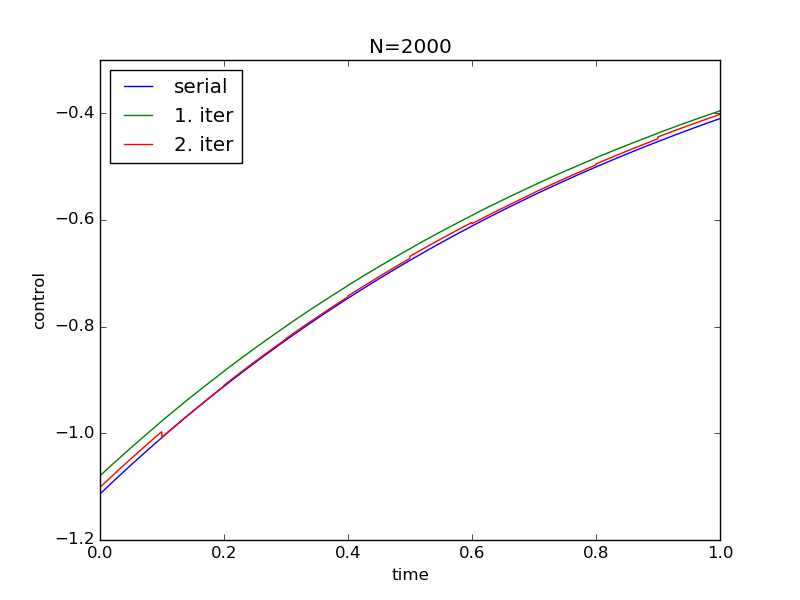
\includegraphics[width=\linewidth]{mufail2000.png}
  \caption{The second iteration gives a solution closer to the non-penalty solution, as we would expect. However the control from the second iteration is less smooth than the control from the first iteration.}
  \label{Fig 1}
\end{figure}

\begin{figure}
  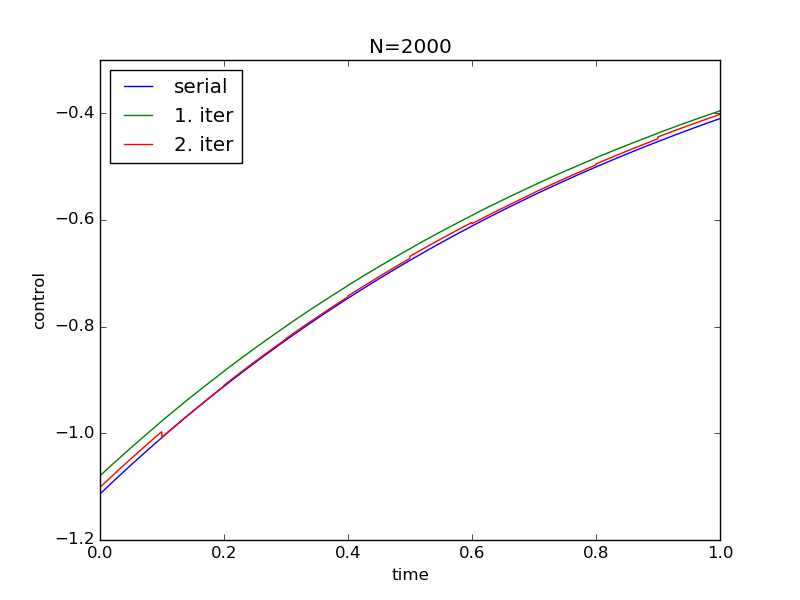
\includegraphics[width=\linewidth]{mufail2000.png}
  \caption{We see the same as for the $N=2000$ case. }
  \label{Fig 2}
\end{figure}
\begin{center}
    \begin{tabular}{| l | l | l |}
    \hline
     & iterations L-BFGS & iterations  L-BFGS + $\mu$-trick \\ \hline
    $N=2000$ and $\mu=0.1N$ &  15 & 15 \\ \hline
    $N=2000$ and $\mu=0.5N$&  16 &  28	\\ \hline
    $N=3000$ and $\mu=0.1N$ &  15 & 15 \\ \hline
    $N=3000$ and $\mu=0.5N$&  27 &  28	\\ \hline
    \end{tabular}
\end{center}
I also added plots of the controls I get from solving the problem using the $\mu$-trick compared with the control we get from not using any penalties. What both the iteration count and plots tells us is that the $\mu$-trick is not working very well. The number of iterations using is either the same or bigger than what we see for not using old Hessian. From the plots we also see that the solutions gets less smooth and distorted when using the $\mu$-trick. I have also done other tests, and they all yield similar results. 
\\
\\
\textbf{L-BFGS memory}
\\
Doing tests I noticed that the number of iterations needed for the L-BFGS to converge were dependent on the memory of the method. By memory I mean the number of iterations the approximation of the inverted Hessian were based on. I tested the problem stated above with $N=1000$, for different number of processes, and for different L-BFGS memory size. Below I have added a table that tells us the number of iteration required for the method to converge for different combinations of number of processes and memory.

\begin{center}
    \begin{tabular}{| l | l | l |}
    \hline
    m\textbackslash L-BFGS memory & $mem=m$& $mem=2m$ \\ \hline
    $m=2$  &  3 & 3 \\ \hline
    $m=5$  &  12 &  9	\\ \hline
    $m=10$ &  Fail & 14 \\ \hline
    $m=15$ &  32 &  19	\\ \hline
    $m=20$ &  42 & 24 \\ \hline
    $m=30$ &  61 &  34	\\ \hline
    \end{tabular}
\end{center}
If we solve this problem without using any penalties, we need two iterations. This means, that if we assume no overhead and perfect scaling and so on, we get faster execution using the penalty method, than the serial situation.
\\
\\
\textbf{Relation between $\mu$ and number of processes $m$}
\\
If we let $\mu$ and the number of discretization points $N$ be constant, and then increase the number of processes $m$, we see that the penalty solution deviates from the serial solution. If we instead let the relation $\frac{N}{m}=C$, and set $\mu = \alpha C$, we see that the resulting control of the penalty method are similar for different $m$'s. Illustrate this with test results using $C=200$, and increasing $N$:
\begin{figure}
  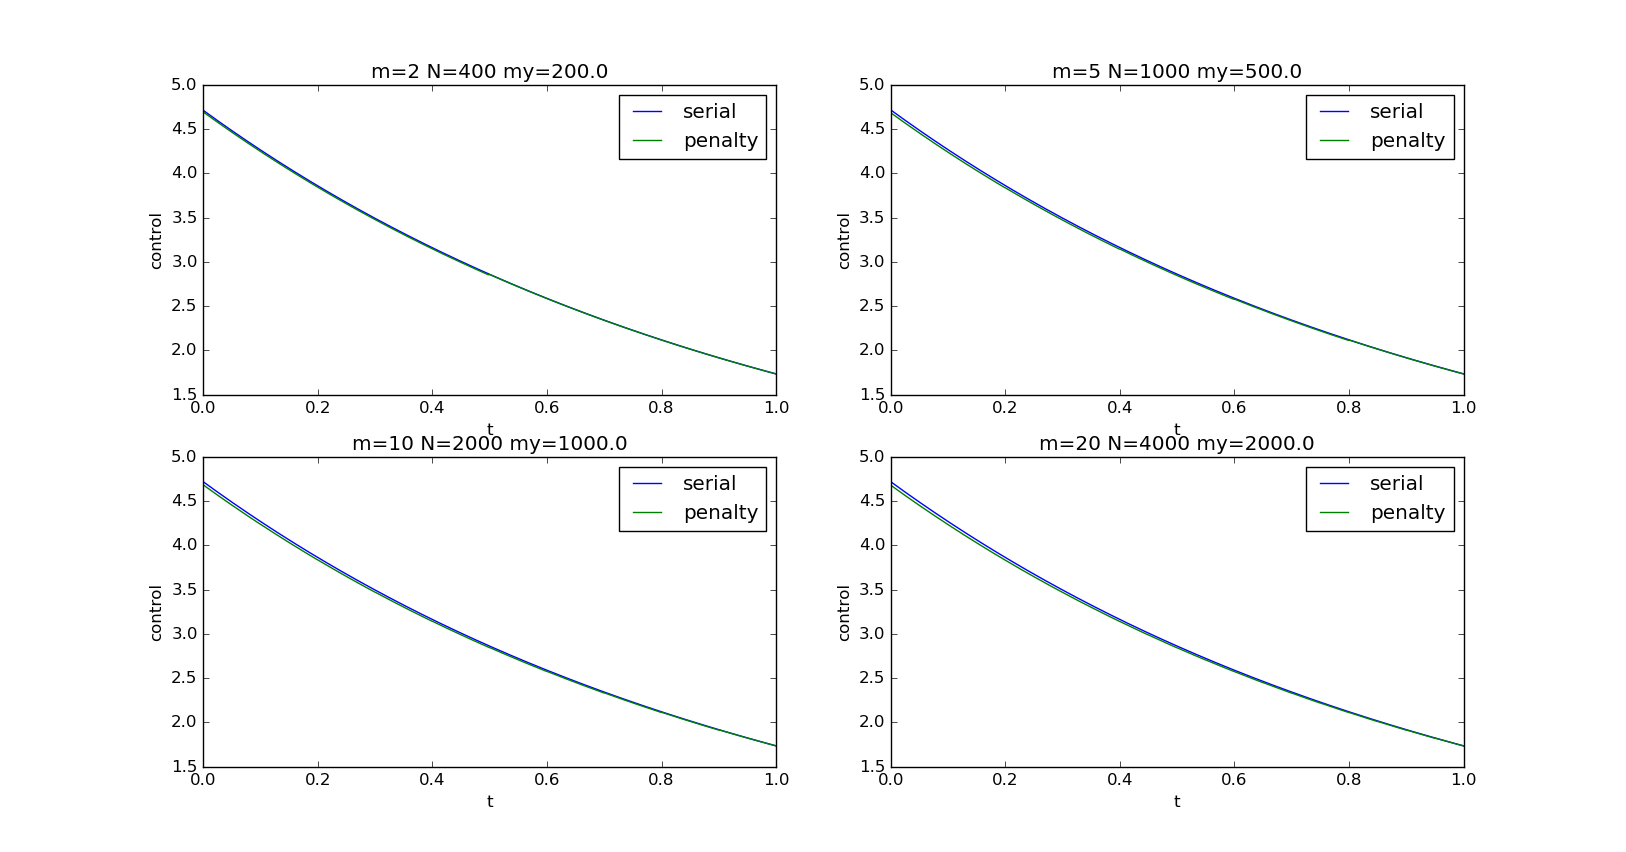
\includegraphics[width=\linewidth]{Mu_mRelation.png}
  \caption{Testing penalty method with different number of processes, and letting $\frac{N}{m}=200$. Notice that this yields very similar controls. }
  \label{Fig 3}
\end{figure}
\begin{center}
    \begin{tabular}{| l | l | l | l |}
    \hline
     & $N$ & iterations & $||\text{penalty}-\text{serial} ||_{L^2} $  \\ \hline
    $m=2$  &  400 & 3 & 1.11e-04  \\ \hline
    $m=5$  &  1000 &  9&	3.34e-04 \\ \hline
    $m=10$ &  2000 & 14&  4.07e-04\\ \hline
    $m=20$ &  4000 &  25	& 5.07e-04\\ \hline
	\end{tabular}
\end{center} 
\textbf{More iterations}
\\
Tried solving the problem using functional 
\begin{align*}
J(u,y)=\int_0^T (C_0u(t)-C_1)^2dt + (y(T)-y_T)^2
\end{align*}
This resulted in more iterations for the serial L-BFGS. Results for $C_0=2 $ and $C_1= 1000$ can be found below:
\begin{center}
    \begin{tabular}{| l | l | l |}
    \hline
    m\textbackslash L-BFGS memory & $mem =\max(m,10)$& $mem=2max(m,10)$\\ \hline
    $m=1$  &  5 &  \\ \hline
    $m=2$  &  6 &  6	\\ \hline
    $m=4$ &  8 & 8 \\ \hline
    $m=8$ &  Fail &  12	\\ \hline
    $m=16$ &  Fail & 21 \\ \hline
    $m=32$ &  Fail &  39	\\ \hline
    \end{tabular}
\end{center}
Results for for $C_0=0.1 $ and $C_1= 100$:
\begin{center}
    \begin{tabular}{| l | l | l |}
    \hline
    m\textbackslash L-BFGS memory & $mem =\max(m,10)$& $mem=2max(m,10)$\\ \hline
    $m=1$  &  11 &  \\ \hline
    $m=2$  &  Fail &  12	\\ \hline
    $m=4$ &  Fail & Fail \\ \hline
    $m=8$ &  Fail &  28	\\ \hline
    $m=16$ &  Fail & 35 \\ \hline
    $m=32$ &  Fail &  51	\\ \hline
    \end{tabular}
\end{center}
Results for for $C_0=2 $ and $C_1= -1$:
\begin{center}
    \begin{tabular}{| l | l | l |}
    \hline
    m\textbackslash L-BFGS memory & $mem =\max(m,10)$& $mem=2max(m,10)$\\ \hline
    $m=1$  &  4 &  \\ \hline
    $m=2$  &  5 &  5	\\ \hline
    $m=4$ &  17 & 17 \\ \hline
    $m=8$ &  22 &  20	\\ \hline
    $m=16$ &  51 & 28 \\ \hline
    $m=32$ &  100 &  43	\\ \hline
    \end{tabular}
\end{center}
\textbf{Non-linear example}
\\
To make the problem more difficult we can change the functional by increasing the power of the $y(T)-yT$ term in the following way:
\begin{align*}
J(u,y) = \int_0^T (C_0u(t)-C_1)^2dt + \frac{1}{4}(y(T)-y_T)^4
\end{align*}
When doing this one need to change the adjoint equation, but it is quite simple. Here is a result of solving this problem using $C_0=1 $ and $C_1= 0.5$:
\begin{center}
    \begin{tabular}{| l | l | l |}
    \hline
    m\textbackslash L-BFGS memory & $mem =\max(m,10)$& $mem=2max(m,10)$\\ \hline
    $m=1$  &  14 &  \\ \hline
    $m=2$  &  16 & 21 	\\ \hline
    $m=4$ &  22 & 21 \\ \hline
    $m=8$ &  Fail &  28	\\ \hline
    $m=16$ &  Fail & 28 \\ \hline
    $m=32$ &  124 &  52	\\ \hline
    \end{tabular}
\end{center}
\begin{figure}
  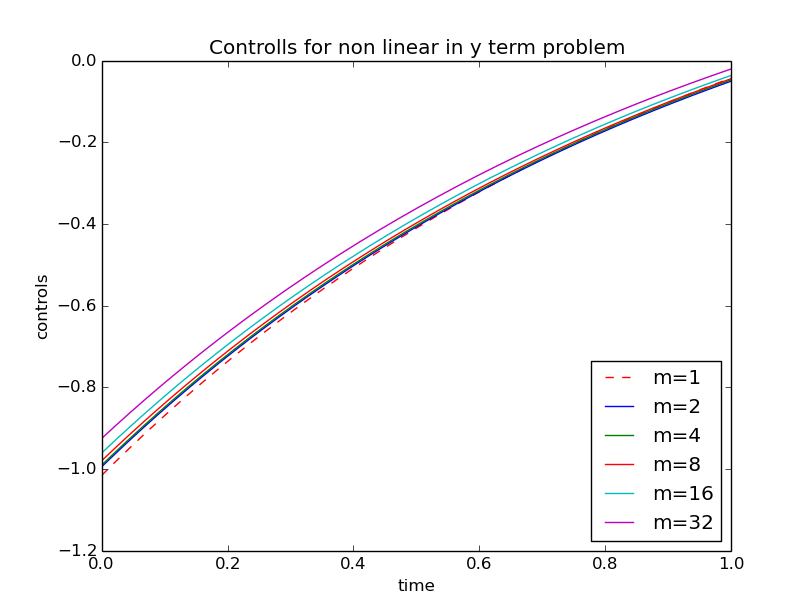
\includegraphics[width=\linewidth]{non_linY.png}
  \caption{Plot of control for different m values, that are the result of the non-linear problem I have iteration results for above. }
  \label{Fig 4}
\end{figure}
\end{document}